The grader makes the following procedure call:

\texttt{find\_best(8)}

There are $n = 8$ boxes. Suppose the prize types are $[3,2,3,1,3,3,2,3]$.
All possible calls to the procedure `ask' and the corresponding return values are listed below.

\begin{itemize}
\item `ask(0)' returns $[0, 3]$
\item `ask(1)' returns $[0, 1]$
\item `ask(2)' returns $[1, 2]$
\item `ask(3)' returns $[0, 0]$
\item `ask(4)' returns $[2, 1]$
\item `ask(5)' returns $[2, 1]$
\item `ask(6)' returns $[1, 0]$
\item `ask(7)' returns $[3, 0]$
\end{itemize}

In this example, the diamond is in box $3$. So the procedure \texttt{find\_best} should return $3$.

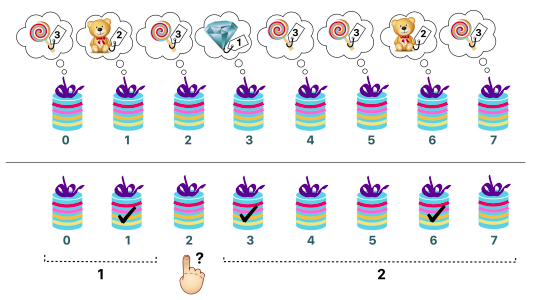
\includegraphics{prize.png} 

The above figure illustrates this example. The upper part shows the types of the prizes in each box. The lower part illustrates the query \texttt{ask(2)}. The marked boxes contain more expensive prizes than the one in box $2$.